\Section{Прикладные протоколы}{Лекции 7-8}{Игорь Смирнов}

\begin{itemize}
    \item Удалённые терминалы
    \item Электронная почта
    \item Передача файлов
    \item Передача новостей
    \item Обмен мгновенными сообщениями
    \item Передача объектов
    \item ...
\end{itemize}

\Subsection{Протоколы удалённых терминалов}

\begin{itemize}
    \item Rlogin
    \item TELNET~--- не использует шифрование, логины и пароли передаются по HTTP в открытом виде. У него есть и вторая роль: он может быть использован как универсальный TCP-клиент для большинства протоколов. Например, если у вас нет почтового клиента, но вы наизусть помните почтовый протокол, вы можете с помощью TELNET подключиться к электронной почте и вручную, набирая команды и анализируя ответы, общаться с электронной почтой (очень полезно)
    \item ssh~--- заменил TELNET. Обеспечивает полное шифрование
    \item X-протокол. Графическая распределённая среда. Есть клиент и удалённый сервер. На сервере ОС с графической оболочкой, окна которой мы хотим отображать на клиенте (например, так можно запустить старый виндовый калькулятор). Он передаёт не графические объекты, а цепочку событий. Запускается поверх ssh.
\end{itemize}

\Subsection{Электронная почта}

Архитектура почты следующая: у нас есть несколько почтовых серверов. Каждый из серверов имеет базу почтовых ящиков. В тот момент, когда клиент хочет передать почту, он обращается к своему серверу, передаёт ему почту с помощью протокола SMTP. Дальше почтовый сервер определяет, какому серверу это послать и посылает по SMTP. Когда второй пользователь хочет прочитать почту, он обращается к своему серверу по протоколу POP-3 или IMAP-4 к своему ящику.

Формат почтового адреса: {\tt name@host.domain}
\begin{itemize}
    \item name:
    \begin{itemize}
        \item Имя пользователя
        \item Название почтового ящика
        \item Название списка рассылки
    \end{itemize}
\end{itemize}

Сама по себе электронная почта позволяет передавать только текст. Ни картинки, ни компьютерную графику не передать.

Но часто мы хотим передавать котиков. Поэтому разработали стандарт MIME~--- расширение электронной почты. Он позволяет закодировать в тексте нетекстовую информацию.

\Subsubsection{Протокол SMTP}

Для передачи почты используется SMTP~--- простой протокол передачи почты. Заменил протокол MTP.

Было несколько расширений. Добавили, например, аутентификацию. 

Протокол поддерживает обмен данными между клиентом и почтовым агеном и обмен данными между двумя почтовыми агентами.

Использует TCP (порт 25).

Не поддерживает шифрования.

Базовая версия не поддерживает аутентификацию. То есть раньше любой человек мог послать письмо от имени любого человека.

Это текстовый протокол. То есть и команды клиента передаются в текстовом виде, и ответы сервера передаются в текстовом виде. Сделано это для простоты.

Договорились, что формат ответа сервера следующий: код XYZ, а дальше текстовое сообщение.

X~--- 1, если это информационное сообщение, 2~--- всё хорошо, 3~--- warning, 4~--- ошибка клиента, 5~--- ошибка сервера.

Соединение:
\begin{itemize}
    \item 220~--- всё хорошо
    \item 554~--- сервер не готов с вами общаться
\end{itemize}

HELO <домен>:
\begin{itemize}
    \item 250~--- всё хорошо
    \item 504, 550~--- домен не поддерживается
\end{itemize}

MAIL FROM: <адрес>:
\begin{itemize}
    \item 250
    \item 552, 451, 452, 550, 553, 503
\end{itemize}

RCPT TO: <адрес>:
\begin{itemize}
    \item 250, 251
    \item 550, 551, 552, 553, 450, 451, 452, 503, 550
\end{itemize}

DATA

кидает ворнинг 354 (или ошибку 451, 554, 503, если что-то пошло не так), потом вводим текст письма и заканчиваем его точкой на пустой строке.

Если всё хорошо, получим 250, иначе~--- 451, 554, 503

NOOP~--- нет операции
\begin{itemize}
    \item 250
\end{itemize}

QUIT
\begin{itemize}
    \item 221
\end{itemize}

Но где указывать subject и всё такое? В тексте письма! В RFC прописано, где и что должно идти.

Расширение~--- ESMTP

EHLO~--- этот сервер поддерживает или не поддерживает ESMTP
\begin{itemize}
    \item 250
    \item 504, 550
\end{itemize}

VRFY <mailbox>~--- существует ли почтовый ящик
\begin{itemize}
    \item 250, 251, 252
    \item 550, 551, 553, 502, 504
\end{itemize}

EXPN <maillist>~--- список рассылки
\begin{itemize}
    \item 250, 252
    \item 550, 500, 502, 504
\end{itemize}

Но эти две команды как будто специально сделаны для спамеров. Поэтому не используются.

RSET~--- прерывает текущую процедуру посылки сообщения
\begin{itemize}
    \item 250
\end{itemize}

{\bf Аутентификация.}

Реализуется как расширение SMTP. Ответ на EHLO~--- список поддерживаемых механизмов.

Механизмы аутентификации:
\begin{itemize}
    \item KERBEROS\_4
    \item GSSAPI
    \item S/KEY
\end{itemize}

Есть два способа провести аутентификацию: с помощью AUTH и с помощью MAIL FROM.

AUTH <механизм> [<строка>]
\begin{itemize}
    \item 334
    \item 504, 503
\end{itemize}

Секция команды MAIL FROM:
\begin{itemize}
    \item MAIL FROM: <адрес> AUTH=строка
    \item MAIL FROM: <адрес> AUTH=<>
    \item Используется для передачи идентификационной строки сообщения в <<доверительных>> сообществах
\end{itemize}

Ещё когда-то пользовались способом POP3 before SMTP. В POP3 аутентификация была с самого начала.

Хотим послать почту от пользователя Пупкин. Регистрируемся по POP3 на этом сервере. Потом с этого же сокета делаем SMTP соединение.

{\bf Маршрутизация.}

Раньше мы говорили, что почта от исходного сервера передаётся на сервер получателя. Но в некоторых случаях нам хочется направлять почту через определённые серверы (например, для буферизации).

{\bf Кулстори.} Компания Proctor\&Gamble, 2001 год. Секретарша послала письмо своей подруге о том, что она приглашает её на вечеринку. По ошибка она нажала кнопку не <<послать подруге>>, а <<послать почту всем>>. И все пользователи получили это письмо. Дальше, возмущённые таким использованием корпоративной почты, написали ей ответ: <<Уважаемая, не нужно использовать электронную почту для массовых рассылок>>. Примерно 10\% из отвечавших случайно нажали кнопку <<Ответить всем>>. На третьей итерации ситуация была такая же. На несколько дней была выведена сеть, потому что все серверы занимались только тем, что передавали одинаковые сообщения друг другу.

Мораль: трафиком хочется управлять. 

Расширяются команды MAIL FROM и RCPT TO:
\begin{itemize}
    \item RCPT TO: <@first.com, @second.ru, ivan@gmail.com>
    \item MAIL FROM: <@first.ru, peter@mail.ru>
    \item Адреса серверов перемещаются из одного списка в другой
\end{itemize}

То есть почта сначала попадёт в @first.com, потом в @second.ru, а уже потом в @gmail.com.

А в MAIL FROM в обратном порядке записываем уже пройденные, чтобы в обратную сторону можно было повторить тот же процесс.

{\bf Стандарт MIME.}

Интерпретирование текста сообщения как структурированную базу с вложениями и всем таким.

Используется два способа кодирования:
\begin{itemize}
    \item BASE64~--- давайте выделим 64 символа, которые точно не будут изменяться и будем кодировать ими все 256 символов.\\
    a-z, A-Z, 0-9, +-\\
    Их можно закодировать 6 битами. Закодируем исходное сообщение ими.\\
    Таким образом, почта становится больше в 4/3 раза. То есть если мы захотим передать файл в 9 Мб, на самом деле будет передаваться 12 Мб.
    \item Quoted-printable\\
    Вместо любого символа, берём его код в 16-ричном виде {\tt =AF=60=FF}.\\
    Трафика в 3 раза больше. Но при этом быстрее обрабатывать.
\end{itemize}

Формат заголовков в MIME:\\
{\tt =? Charset ? Encoding ? Encoded-text ?=}
\begin{itemize}
    \item Charset~--- набор символов
    \item Encoding~--- кодировка
    \begin{itemize}
        \item B~--- BASE64
        \item Q~--- Quoted-Printable
        \item Encoded-text~--- текст заголовка
    \end{itemize}
\end{itemize}

Пример:\\
{\tt Subject: Re: =?koi8-r?b?y8zVwg==?=}

\begin{figure}[H]
  \centering
  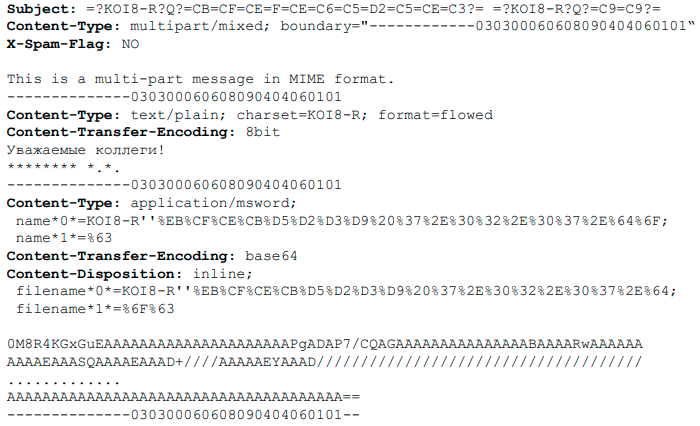
\includegraphics[width=15cm]{images/07/01}
\end{figure}

\Subsubsection{Борьба со спамом}

Сейчас будем говорить о технологиях, которые не позволяют пользователям посылать почту от имени другого человека (mail spoofing).

\begin{itemize}
    \item SPF (Sender Policy Framework) 
    \item Caller ID for E-mail 
    \item Sender ID~--- объединение технологий:
\end{itemize}

Идея Sender ID: владелец домена публикует в открытом доступе список адресов, с которых можно отправлять почту от имени данного домена. Например, <<Почту Mail.ru можно отправлять только используя SMTP сервер mail.ru>>.

Получатель проверяет сообщение, руководствуясь заголовками письма и записями о разрешённых именах домена.

Purported Responsible Address (PRA)~--- предполагаемый адрес отправителя.

Задача~--- извлечение PRA и проверка по базе разрешённых адресов.

Информация о разрешённых адресах домена хранится в DNS (в записи TXT).

PRA ищется по заголовкам письма. Если найден, то на основе PRA определяется PRD (Purported Responsible Domain).

Запрашиваем DNS сервер, отвечающий за домен PRD и принимаем решение о дальнейших действиях.

Если PRA не был найден, то письмо посылается на дополнительную проверку.

\Subsubsection{Протокол POP-3}

Post Office Protocol~--- протокол доступа к почтовому ящику.

Позволяет аутентифицировать пользователя, посмотреть список писем, скопировать письма в локальный ящик и удалять письма с сервера.

Ящик~--- одна почтовая папка (Inbox).

Транспорт~--- TCP (порт 110).

Не шифрованный.

{\bf Команды.}

USER <имя>
\begin{itemize}
    \item -ERR~--- если не поддерживается plaintext authentication
    \item +OK~--- в остальных случаях
\end{itemize}

Если такого пользователя в системе нет, получаем ответ OK, чтобы хакеры не смогли проверить, есть ли пользователь.

PASS <пароль>
\begin{itemize}
    \item -ERR~--- неуспешная аутентификация
    \item +OK~--- успешная аутентификация
\end{itemize}

STAT
\begin{itemize}
    \item +OK <N> <M>~--- N писем общей длиной M
\end{itemize}

LIST~--- пролистать список писем
\begin{itemize}
    \item +OK\\
    1 <длина 1>\\
    ...\\
    N <длина N>
\end{itemize}

Это чтобы показывать прогресс бар.


LIST <N>
\begin{itemize}
    \item +OK\\
    N <длина>
    \item -ERR~--- сообщение отсутствует
\end{itemize}

RETR <N>~--- получение письма
LIST~--- пролистать список писем
\begin{itemize}
    \item +OK\\
    <текст сообщения>\\
    .
    \item -ERR~--- сообщение отсутствует
\end{itemize}

DELE <N>~--- помечает письмо флагом на удаление. А реальное удаление происходит при завершении транзакции.
\begin{itemize}
    \item +OK
    \item -ERR~--- сообщение отсутствует
\end{itemize}

RSET~--- сброс транзакции

QUIT~--- выполнение транзакции и разрыв соединения

В следующих стандартах появилось ещё несколько команд:

TOP <N> <M>~--- превьюшки писем
\begin{itemize}
    \item +OK\\
    <заголовок сообщения N>\\
    <пустая строка>\\
    <M строк сообщения>
    \item -ERR~--- сообщение отсутствует
\end{itemize} 

UIDL <N>~--- посмотреть идентификатор письма, который ему присвоил почтовый сервер
\begin{itemize}
    \item +OK <N> <UID>
    \item -ERR~--- сообщение отсутствует
\end{itemize} 

UIDL
\begin{itemize}
    \item +OK\\
    1 <UID 1>\\
    2 <UID 2>\\
    ...
\end{itemize} 

Позволяет скачивать только новые письма.

APOP <имя> <дайджест>
\begin{itemize}
    \item +OK
    \item -ERR~--- ошибочная аутентификация
\end{itemize} 

Дайджест вычисляется по алгоритму MD5.

В вычислении используется строка сервера <pid.clock@hostname>

Достоинства POP-3:
\begin{itemize}
    \item Простота реализации
    \item Большая распространённость
\end{itemize}

Недостатки POP-3:
\begin{itemize}
    \item Отсутствие шифрования
    \item Аутентификация
    \item Блокировка ящика (нельзя двум клиентам подключиться к одному ящику)
    \item Отсутствие папок
    \item Отсутствие атрибутов сообщения
\end{itemize}

\Subsubsection{Протокол IMAP-4}

Создан как альтернатива POP-3.

Особенности IMAP-4:
\begin{itemize}
    \item Позволяет хранить удаленную структуру папок сообщений
    \item Обеспечивает асинхронный обмен командами
    \item Уникальный номер команды и ответа
    \item Флаги сообщений
    \item Уникальные идентификаторы сообщений
    \item Механизмы копирования и перемещения сообщений
    \item Средства поиска сообщений
    \item Варианты аутентификации (login и authenticate)
    \item Использует протокол TCP, порт №143
\end{itemize}

{\bf Флаги сообщений}

Можно использовать системные и пользовательские флаги.

Системные флаги:
\begin{itemize}
    \item $\backslash$Seen
    \item $\backslash$Answered
    \item $\backslash$Deleted
    \item $\backslash$Draft
    \item $\backslash$Recent
\end{itemize}

{\bf Команды.}

На всех стадиях:
\begin{itemize}
    \item CAPABILITY~--- запрос списка возможностей
    \item NOOP
    \item LOGOUT
\end{itemize}

Стадия <<Неаутентифицирован>>
\begin{itemize}
    \item LOGIN <username> <password>
    \item AUTHENTICATE <method>
\end{itemize}

Стадия <<Аутентифицирован>>:
\begin{itemize}
    \item SELECT <имя\_ящика>~--- выбор ящика
    \item EXAMINE <имя\_ящика>~--- выбор ящика (RO)
    \item CREATE <имя\_ящика>~--- создание ящика
    \item DELETE <имя\_ящика>~--- удаление ящика
    \item RENAME <старое\_имя> <новое\_имя>~--- переименование ящика
    \item SUBSCRIBE <имя\_ящика>~--- подписка на ящик
    \item UNSUBSCRIBE <имя\_ящика>~--- отмена подписки на ящик
    \item LIST <база> <имя\_ящика>~--- выдача списка ящиков
    \item LSUB - <база> <имя\_ящика>~--- выдача списка подписанных ящиков
    \item STATUS <имя\_ящика> [<имена\_элтов\_состояния>]~--- выдача состояния ящика
    \item APPEND <имя\_ящика> [(флаги)] [...]~--- добавить сообщение в ящик
\end{itemize}

Стадия <<Выбран>>:
\begin{itemize}
    \item CHECK~--- проверка ящика
    \item CLOSE~--- удаление помеченных сообщений и закрытие ящика
    \item EXPUNGE~--- удаление помеченных сообщений
    \item SEARCH [CHARSET] <критерии>~--- поиск сообщения
    \item FETCH <набор\_сообщений> <эл-ты данных>
    \item STORE <набор\_сообщений> <значение>~--- изменение флагов сообщений
    \item COPY <набор\_сообщений> <имя\_ящика>~--- копирование сообщений в ящик
    \item UID <команда>~--- выдача идентификаторов сообщений
\end{itemize}

{\bf Отклики.}

В отличие от POP-3, где откликов всего 2 (OK и ERR), тут их много. Некоторые из них могут быть асинхронными.

\Subsection{Протоколы передачи файлов. FTP}

\begin{itemize}
    \item sftp~--- TCP
    \item tftp~--- UDP
    \item ftp~--- TCP
\end{itemize}

FTP использует двухканальную передачу данных, поэтому у него используется два порта: 21 и 20.

FTP поддерживает активный и пассивный режимы передачи.

Двухканальная система передачи:
\begin{itemize}
    \item Управляющий канал
    \begin{itemize}
        \item Предназначен для передачи команд
        \item Существует всё время обмена
    \end{itemize}
    \item Канал данных
    \begin{itemize}
        \item Предназначен для передачи файлов и каталогов
        \item Организуется на время передачи
        \item Используется порт 20 или непривилегированный порт
    \end{itemize}
\end{itemize}

\Subsubsection{Активный режим}

Режим <<по умолчанию>>.

Канал передачи данных инициируется сервером.

Клиент открывает слушающий порт и ждёт подсоединения сервера.

Невозможно использовать NAT, Proxy.

Обычно запрещён в межсетевых экранах.

Данные могут передаваться в любую сторону (как с клиента на сервер, так и наоборот).

\Subsubsection{Пассивный режим}

Клиент инициирует соединение данных. Сервер просто говорит, на каком номере порта он ждёт соединение.

Сервер открывает слушающий порт.

Поддерживается не всеми реализациями.

\Subsubsection{Команды}

\begin{itemize}
    \item USER <имя>
    \item PASS <пароль>
    \item REIN~--- реинициализация
    \item ABOR~--- прервать обмены
    \item QUIT
    \item DELE <имя>~--- удалить файла
    \item RNFR <имя>~--- переименовать из
    \item RNTO <имя>~--- переименовать в
    \item CWD <путь>~--- сменить каталог
    \item CDUP~--- перейти в родительский каталог
    \item RMD <имя>~--- удалить каталог
    \item MKD <имя>~--- создать каталог
    \item PWD~--- показать текущий каталог
    \item PORT a1, a2, a3, a4, p1, p2 - перевод сервера в активный режим\\
    Address = 'a1.a2.a3.a4'\\
    Port = p1*256+p2
    \item PASV~--- перевод сервера в пассивный режим\\
    227 a1, a2, a3, a4, p1, p2
    \item TYPE \{A|E|I\} – представление информации
    \begin{itemize}
        \item A~--- ASCII
        \item E~--- EDCDIC
        \item I~--- Image
    \end{itemize}
    \item MODE \{S|B|C\} – режим передачи данных
    \begin{itemize}
        \item S~--- Stream
        \item B~--- Block
        \item C~--- Compressed
    \end{itemize}
    \item RETR <имя>~--- получить файл
    \item STOR <имя>~--- записать файл
    \item LIST [<путь>]~--- получить список файлов с атрибутами
    \item NLST [<путь>]~--- получить список имен файлов
\end{itemize}

Хотим перегнать файл с сервера 1 на сервер 2. Но при этом не хотим сохранять его к себе. 

Это можно устроить с помощью ftp. В командах PORT и PASV мы указывали IP-адрес. С помощью этой махинации, можно сделать так, чтобы серверы передавали файлы друг другу.

Откроем два канала связи. Один сервер переведём в активный режим, а другой в пассивный. Одному передадим команду на посылку данных, а другому на получение.

Но этот способ не всегда работает, потому что злоумышленники могут использовать его для анонимного сканирования портов.

Достоинства FTP:
\begin{itemize}
    \item Эффективность
    \item Гибкость
\end{itemize}

Недостатки:
\begin{itemize}
    \item Не поддерживает шифрования
    \item Не поддерживает безопасной аутентификации
    \item Не поддерживает адресации по URL
    \item Сложность работы с защищёнными сетями
\end{itemize}

\Subsection{Протокол HTTP}

Это протокол передачи файлов.

Но ещё используется как протокол передачи объектов и как транспорт для многих разных интересных систем.

FTP позволял передать файлы. Но мировую паутину на нём не сделали. Но там мы соединяемся и занимаем сокет. Он держит соединение. 

В HTTP идея такая: мы сделали запрос, в запросе есть все данные со всеми заголовками. Мы получили ответ и разорвали соединение.

\Subsubsection{Формат HTTP запроса}
\begin{itemize}
    \item <Request-line>~--- строка запроса
    \item <General-header>~--- общий заголовок
    \item <Request-header>~--- заголовок запроса
    \item <Entity-header>~--- заголовок сообщения
    \item <Body>~--- тело
\end{itemize}

\Subsubsection{Строка запроса}

<METHOD> <URL> <HTTP-VERSION> 

Методы:
\begin{itemize}
    \item GET
    \item POST
    \item HEAD
    \item PUT
    \item DELETE
    \item OPTIONS
    \item ...
\end{itemize}

PUT и DELETE используются в системах публикации

Версия: HTTP/1.0 или HTTP/1.1


\Subsubsection{Заголовки}

{\bf Общий заголовок (General-header)}

Присутствует, когда есть тело сообщения

\begin{itemize}
    \item Connection:
    \item Data:
    \item Pragma:
    \item Transfer-encoding:
    \item Upgrade:
    \item no-cache:
    \item ...
\end{itemize}

{\bf Заголовок запроса (Request-header)}

\begin{itemize}
    \item Accept: принимаемый контент
    \item Accept-Charset: принимаемый набор символов
    \item Accept-Encoding: compress, zip
    \item Accept-Language: da, ru
    \item Authorization: basic xxx=******
    \item From:
    \item Host:
    \item If-modified-since:…
    \item Referer:
    \item User-agent:
    \item ...
\end{itemize}

{\bf Кулстори.} По странному стечению обстоятельств, все браузеры сообщают в User-agent, что они Mozilla. И хром, и IE... Пришло это из браузера Netscape передавал код Mozilla и все под него автоматически подстраивались.

{\bf Заголовок сообщения (Entity-header)}

\begin{itemize}
    \item Allow: GET, POST, HEAD
    \item Content-Encoding: x-zip
    \item Content-Language:
    \item Content-Length: 1245
    \item Content-Type: ...text/html; charset=win-1251
    \item Expires:
    \item Last-Modified:
\end{itemize}

\Subsubsection{Формат ответа}

\begin{itemize}
    \item <Status-line>~--- Строка статуса
    \item <General-header>~--- общий заголовок
    \item <Response-header>~--- заголовок ответа
    \item <Entity-header>~--- Заголовок сообщения
    \item <Body>~--- тело
\end{itemize}

{\bf Строка статуса.}

Формат: <HTTP-VERSION> <Code> <Phrase>

Code:
\begin{itemize}
    \item 1xx~--- информационные
    \item 2xx~--- OK
    \item 3xx~--- Переадресация (redirection)
    \item 4xx~--- Ошибка клиента
    \item 5xx~--- Ошибка сервера
\end{itemize}

{\bf Заголовок ответа.}
\begin{itemize}
    \item Location: переадресация
    \item Server: спецификация сервера
    \item WWW-Authenticate: basic realm=’localzone’
    \item Age: Возраст ресурса
\end{itemize}

\Subsubsection{Развитие протокола}

Протокол SPDY разработан в Google. Обеспечивается сжатие, мультиплексированная передача и т.п.. С 2015 года не поддерживается

Протокол HTTP/2.

Создан на основе SPDY в 2015 году.

Основные возможности:
\begin{itemize}
    \item Сжатие данных и заголовков
    \item Мультиплексирование запросов в одном TCP-соединении
    \item Посылка ответов без запросов (в т.ч., опережающая посылка)
    \item Push-уведомления
    \item Приоритизация запросов
    \item Безопасность
\end{itemize}
